\documentclass[xcolor=dvipsnames,11pt]{beamer}   
\usepackage{beamerthemesplit}              %几个有关的宏包
\usepackage{xeCJK}                                    %一般不要轻易删除它们
\usepackage{verbatim}                            %


%\usetheme{Singapore}
\usecolortheme[named=Plum]{structure}
%\useoutertheme{infolines} 

\usetheme[height=7mm]{Rochester}
\setbeamertemplate{items}[ball] 
\setbeamertemplate{blocks}[rounded][shadow=true]

%\useoutertheme{miniframes}
%\setbeamertemplate{navigation symbols}{} 

%\usetheme{Torino}  

   
\usepackage{fontspec}  
\setsansfont{KaiTi} % font name is case-sensitive  
%\usetheme{Goettingen}         

%\setCJKmainfont{SimSun}
%\setCJKfamilyfont{hei}{SimHei}                     %用汉字,定义”kai“为文档字体。


\hypersetup{pdfpagemode={FullScreen}} % 全屏幕




\usepackage{graphicx}
\begin{document}
                                           

\title{Linux内核性能测试框架的实现与优化\\ {\small开题报告}}
\author[杨\ 扬]{杨\ 扬\\指导教师:王生原\ \ 陈渝}
%\author{杨\ 扬}
\institute{清华大学计算机科学与技术系}

\date{2013年3月22日}

\AtBeginSection[]{                              % 在每个Section前都会加入的Frame
          \frame<handout:0>{
            \tableofcontents[current,currentsubsection]
          }
}
\AtBeginSubsection[]                            % 在每个子段落之前
{
          \frame<handout:0>                            % handout:0 表示只在手稿中出现
          {
            %\frametitle{框架}
            \tableofcontents[current,currentsubsection] % 显示在目录中加亮的当前章节
          }
}

\frame{\titlepage}

\section*{目录}                                % section后面加*表示不收录到目录中
\frame {
          \tableofcontents      % 使用这个命令自动生成目录
}


\section{问题定义及背景}
\begin{frame}
\frametitle{背景}

\begin{block}{Linux内核每版本patch数量}
\begin{figure}[htp]
\centering
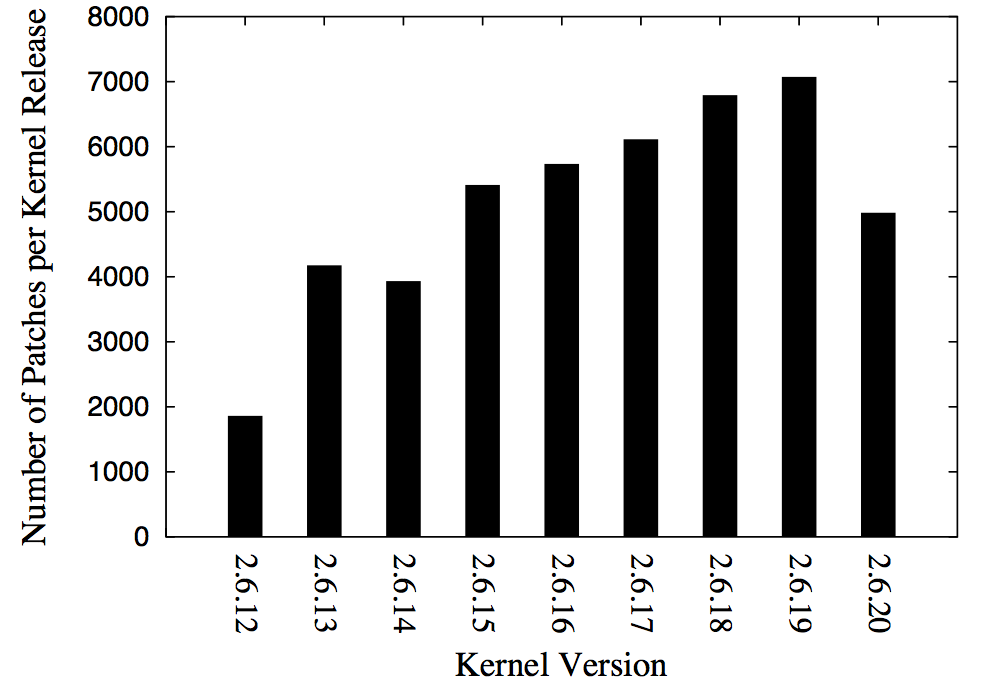
\includegraphics[height=6cm,width=10cm,scale=1.00]{/Users/yy/Pictures/final_paper/pactches_count.png}
\caption{各版本patch数量}
\label{}
\end{figure}
\end{block}
\end{frame}

\begin{frame}
\frametitle{背景(续)}

\begin{block}{Linux开发模式}
\begin{figure}[htp]
\centering
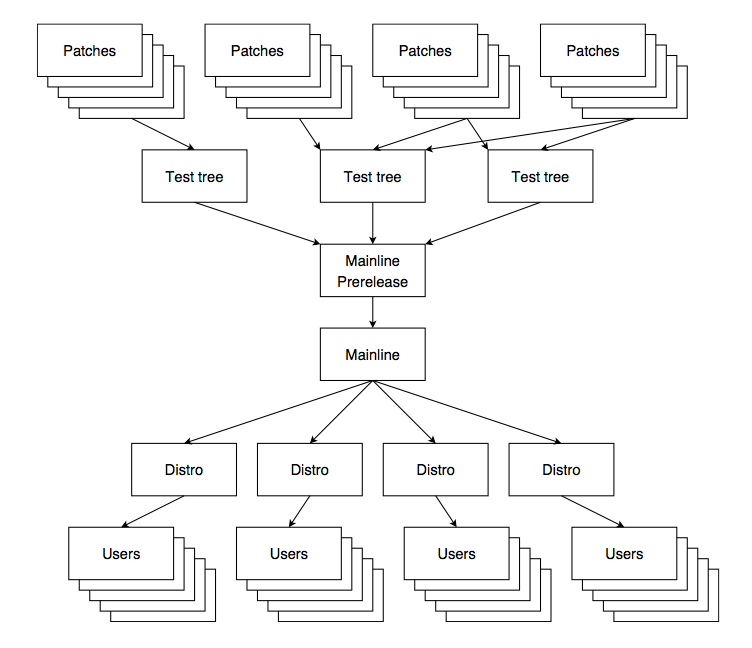
\includegraphics[height=6cm,width=10cm,scale=1.00]{/Users/yy/Pictures/final_paper/linux_kernel_change_flow.png}
\caption{Linux内核的开发模式}
\label{}
\end{figure}
\end{block}
\end{frame}


\begin{frame}
\frametitle{背景(续)}
随着Linux内核开发的全球化,Linux开发的步伐逐渐加快,开发的规模也逐渐扩大,内核开发有以下的特点
\begin{enumerate}
\item 越来越多的新功能被添加到内核中来,导致内核结构越来越复杂
\item 内核复杂的结构使得任何一点改动对内核性能造成影响的可能性加大
\item Linux内核进行官方测试的间隔一般比较大(一般只在有新版本发布的时候才进行比较完整的测试)
\item 一旦有性能损失的问题,这个问题就会随着各大Linux发行版扩散到广大的用户当中并被使用
\end{enumerate}


\end{frame}


\begin{frame}
\frametitle{问题定义}
性能退化(Performance Regression)指的是某些代码提交之后,造成了的性能下降。

开发一套能够进行Linux性能测试的框架,主要有以下特征:
\begin{enumerate}
\item 较快并准确地进行Linux性能测试
\item 在出现performance regression之后,多次运行进行问题的确认
\item 确认performance regression之后,能够最快地定位到出现问题的代码提交
\item 在定位到问题代码之后,将相关的测试数据及出现问题的代码通知给这段代码的作者
\end{enumerate}
\end{frame}


\section{相关工作}
\begin{frame}
\frametitle{相关工作}

\begin{block}{Keeping Kernel Performance from Regressions}
\begin{minipage}[b]{0.30\linewidth}
本文作者为Intel公司的员工,并在文中提到一种比较高效率的查找内核性能下降的测试框架已经发挥了很大的作用,这个测试框架使用Linux的主线代码来进行测试。
\end{minipage}
\begin{minipage}[b]{0.53\linewidth}
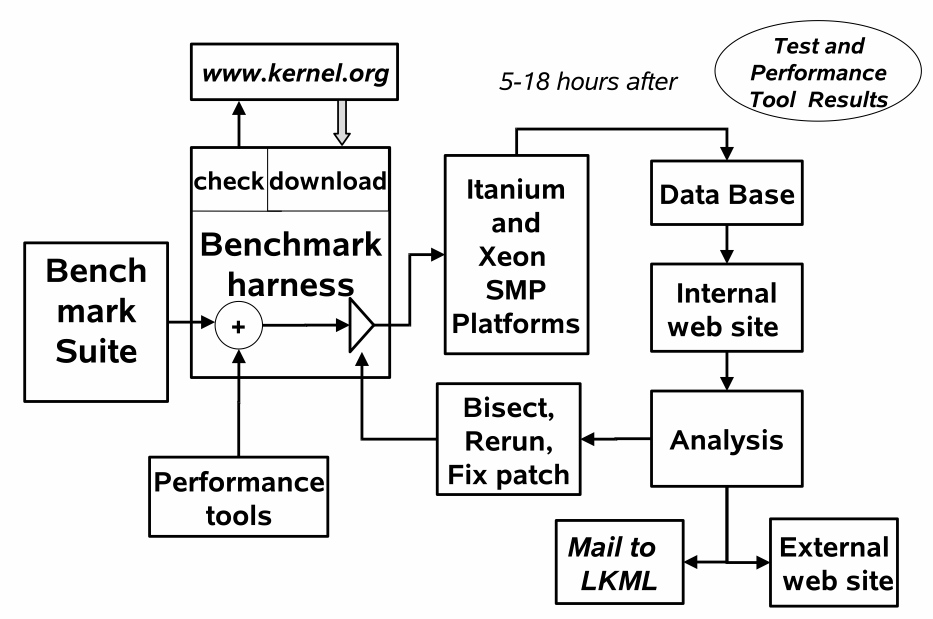
\includegraphics[height=4.8cm]{/Users/yy/Pictures/final_paper/old_lkp_arch.png}
\end{minipage}
\end{block}


\end{frame}

\begin{frame}
\frametitle{相关工作(续)}

\begin{block}{Fully Automated Testing of the Linux Kernel}

\begin{minipage}[b]{0.48\linewidth}
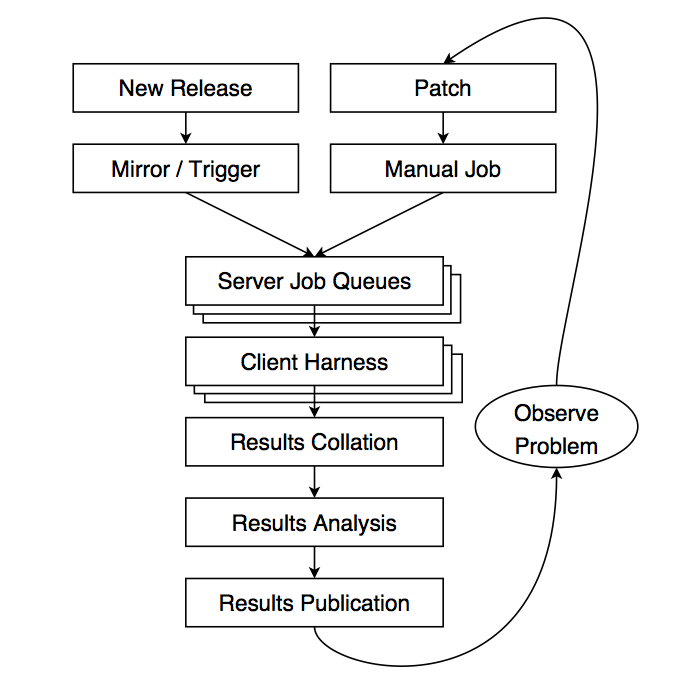
\includegraphics[height=4.8cm]{/Users/yy/Pictures/final_paper/tko_arch.png}
\end{minipage}
\begin{minipage}[b]{0.48\linewidth}
文中提出了对Linux内核进行完整的,全面的测试的测试系统所需要具备的条件:
\begin{itemize}
\item 代码的静态分析
\item  新功能测试
\item  性能测试
\item 压力测试
\end{itemize}

同时,文章中还提到了如何进行有效的测试管理。

\end{minipage}


\end{block}

\end{frame}

\iffalse
\begin{frame}
\frametitle{相关工作(续)}

\begin{block}{Non-scalable locks are dangerous}
在文章中,作者提出了非可扩展锁的使用会在即使很短的临界区内造成整个系统的性能下降,并且通过实验重现了性能下降的场景,并建立模型分析了非可扩展锁造成性能下降的原因。
\end{block}

\begin{block}{Automated Performance Analysis of Load Tests}
作者提出了一种通过分析执行的日志并于上一次的执行结果进行比较的方法来进行负载测试,从而得出对性能负载性能的评测。
\begin{figure}[htp]
\centering
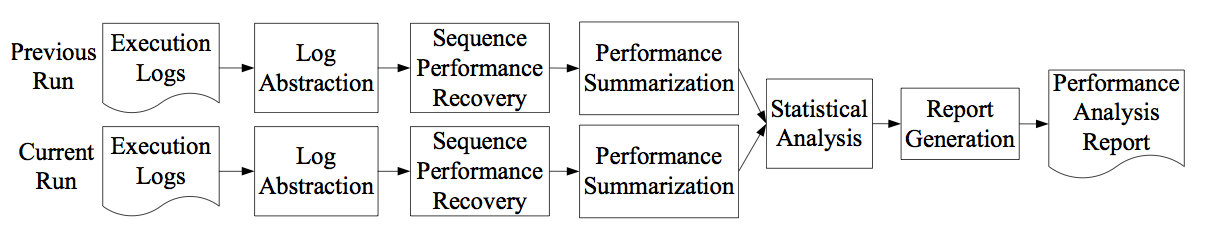
\includegraphics[height=2cm,width=10cm,scale=1.00]{/Users/yy/Pictures/final_paper/auto_perf_anlysis.png}
\caption{自动负载性能分析}
\label{}
\end{figure}
\end{block}

\end{frame}
\fi




\section{框架设计}
\begin{frame}
\frametitle{总体框架设计}
\begin{figure}[htp]
\centering
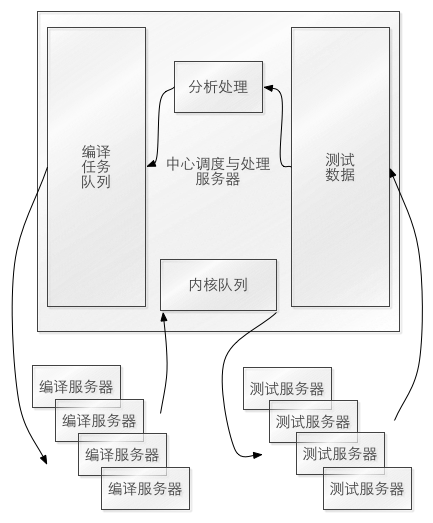
\includegraphics[height=7cm,width=8cm,scale=1.00]{/Users/yy/Pictures/final_paper/total_arch.png}
\caption{总体框架图}
\label{}
\end{figure}
\end{frame}

\begin{frame}
\frametitle{数据流处理}
\begin{figure}[htp]
\centering
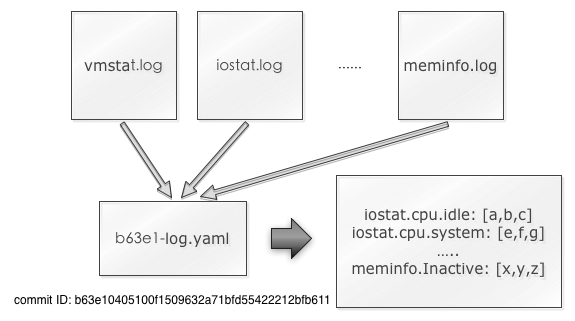
\includegraphics[height=7cm,width=10cm,scale=1.00]{/Users/yy/Pictures/final_paper/data_flow.png}
\caption{数据流处理}
\label{}
\end{figure}
\end{frame}

\begin{frame}
\frametitle{有问题代码的定位(10-Bisect)}
\begin{figure}[htp]
\centering
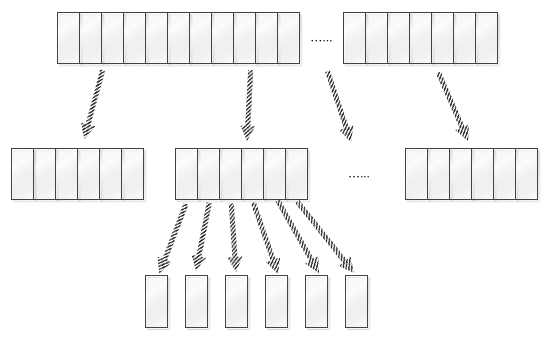
\includegraphics[height=7cm,width=10cm,scale=1.00]{/Users/yy/Pictures/final_paper/10bisect.png}
\caption{10-bisect算法}
\label{}
\end{figure}

\end{frame}


\section{目前进展}

\begin{frame}
\frametitle{目前进展}
目前,我们在该项目中与Intel进行合作,已有的进展是:
\begin{enumerate}
\item Intel工程师吴峰光初步完成了前期框架
\item 已完成大部分系统监视器的编写
\item 已完成大部分系统监视器输出的分析脚本
\item 初步了解了总体框架的运行机制
\end{enumerate}
\end{frame}



\section{工作计划}

\begin{frame}
\frametitle{工作重点}
在我的毕业设计中,我的工作重点主要有以下几点:
\begin{itemize}
\item 理解已有的前期框架
\item 完成系统监视器及相关数据提取
\item 进行数据流格式化及分析
\item 实现用于定位问题代码的10-bisect算法
\end{itemize}



在完成了上面的工作之后,就需要对整个系统进行进一步的优化,使之具有更高的性能和准确度。
\end{frame}

\begin{frame}
\frametitle{工作计划-时间表}
{
\center
\begin{tabular}{c||c}
时间段 & 工作内容\\
\hline
1-4周 & 开题调研及初步设计\\
\hline
5-6周 & 完成系统监视器及相关数据提取\\
\hline
7-8周 & 实现数据流格式化及分析\\
\hline
9-12周 & 实现并调试10-bisect算法\\
\hline
13-15周 & 完成最后的系统调试和优化\\ 
\hline
16周及以后 & 撰写毕业设计论文
\end{tabular}

}
\end{frame}





\frame{
\center \huge \bfseries \color{red} Thank you!\\Q\&A?

}

\end{document}